% --------------------------------------------------------------
% This is all preamble stuff that you don't have to worry about.
% Head down to where it says "Start here"
% --------------------------------------------------------------

\documentclass[12pt]{article}

\usepackage[margin=1in]{geometry}
\usepackage{amsmath,amsthm,amssymb}
\usepackage{graphicx} %This allows to include eps figures
\usepackage{subcaption}
\usepackage[section]{placeins}
\usepackage{layout}
\usepackage{etoolbox}
\usepackage{mathabx}
\usepackage{animate}
\usepackage{array}
\usepackage{siunitx}
% This is to include code
\usepackage{listings}
\usepackage{xcolor}
\definecolor{dkgreen}{rgb}{0,0.6,0}
\definecolor{gray}{rgb}{0.5,0.5,0.5}
\definecolor{mauve}{rgb}{0.58,0,0.82}
\lstdefinestyle{Python}{
    language        = Python,
    basicstyle      = \ttfamily,
    keywordstyle    = \color{blue},
    keywordstyle    = [2] \color{teal}, % just to check that it works
    stringstyle     = \color{green},
    commentstyle    = \color{red}\ttfamily
}

\newenvironment{conditions}
  {\par\vspace{\abovedisplayskip}\noindent\begin{tabular}{>{$}l<{$} @{${}={}$} l}}
  {\end{tabular}\par\vspace{\belowdisplayskip}}

\newcommand{\N}{\mathbb{N}}
\newcommand{\Z}{\mathbb{Z}}

\newenvironment{theorem}[2][Theorem]{\begin{trivlist}
\item[\hskip \labelsep {\bfseries #1}\hskip \labelsep {\bfseries #2.}]}{\end{trivlist}}
\newenvironment{lemma}[2][Lemma]{\begin{trivlist}
\item[\hskip \labelsep {\bfseries #1}\hskip \labelsep {\bfseries #2.}]}{\end{trivlist}}
\newenvironment{exercise}[2][Exercise]{\begin{trivlist}
\item[\hskip \labelsep {\bfseries #1}\hskip \labelsep {\bfseries #2.}]}{\end{trivlist}}
\newenvironment{reflection}[2][Reflection]{\begin{trivlist}
\item[\hskip \labelsep {\bfseries #1}\hskip \labelsep {\bfseries #2.}]}{\end{trivlist}}
\newenvironment{proposition}[2][Proposition]{\begin{trivlist}
\item[\hskip \labelsep {\bfseries #1}\hskip \labelsep {\bfseries #2.}]}{\end{trivlist}}
\newenvironment{corollary}[2][Corollary]{\begin{trivlist}
\item[\hskip \labelsep {\bfseries #1}\hskip \labelsep {\bfseries #2.}]}{\end{trivlist}}



\begin{document}

% --------------------------------------------------------------
%                         Start here
% --------------------------------------------------------------

%\renewcommand{\qedsymbol}{\filledbox}

\title{Assignment 6}%replace X with the appropriate number
\author{Nalet Meinen and Pascal Wyss\\ %replace with your name
Finite Element Analysis I
}
\maketitle

\begin{figure}[!htb]
  \centering
  \vspace*{1cm}
  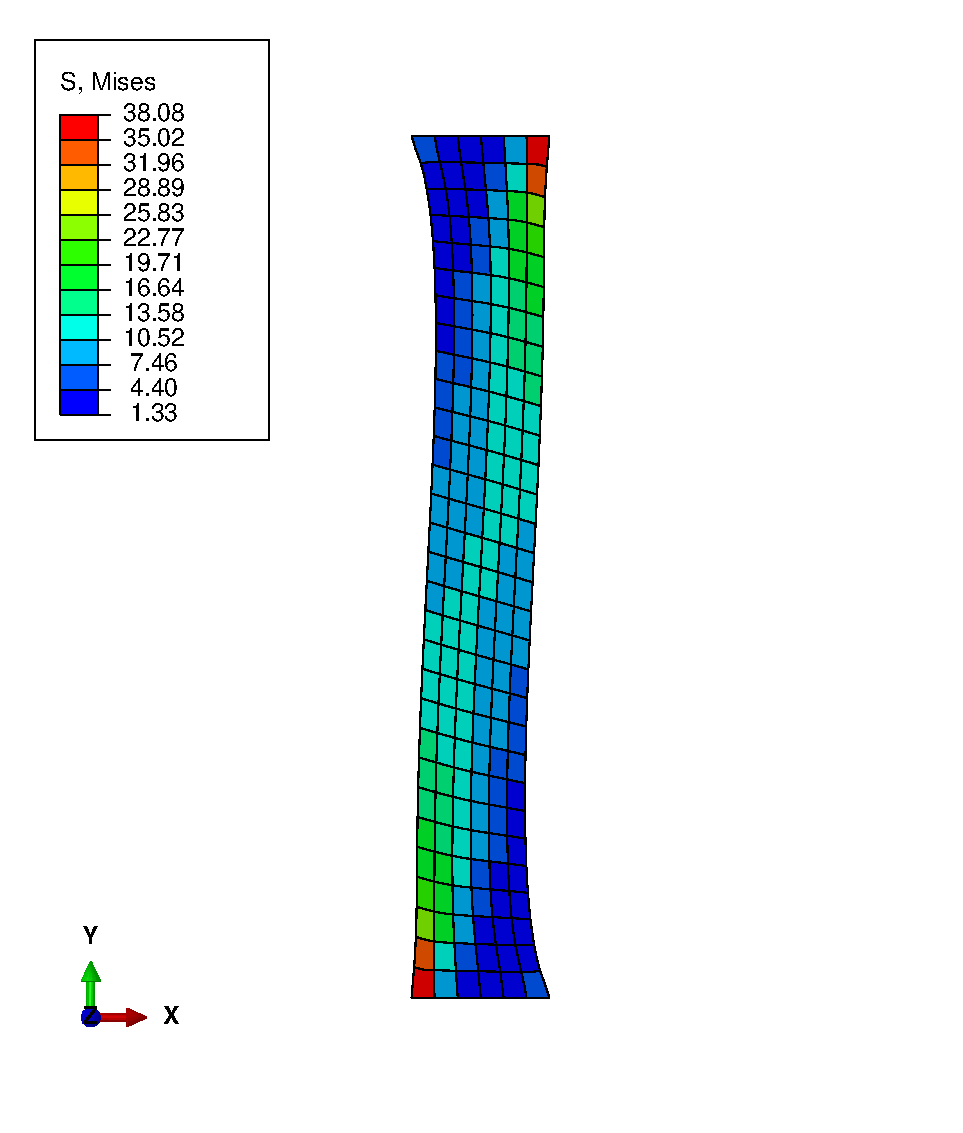
\includegraphics[trim={50mm 20mm 50mm 20mm},clip,width=0.35\linewidth]{pics/s_mises_30}
  \label{fig:0}
\end{figure}

\newpage

\section*{Abstract}
The objective of this assignment is to determine the material parameters. The data is gathered via an anatomical sample during experimental measurements. However, the material parameters cannot be so easily determined by the experimental data. So further analysis is necessary to get a better numerical model that later can be used for further analyzing.
This assignment analyzes the material from the cornea, a part of the eye. The numerical model should give a better understanding of the fibers in the cornea and how they are reacting due to exposes of stresses.


\tableofcontents
\pagebreak
\section{Introduction}
In this assignment, we will create a model that should mimic a part of the cornea. The material of the model in Abaqus should have anisotropic and hyperelastic properties. A good fit for describing this behavior can be made with the Holzapfel-Gasser-Ogden function, which describes very well the strain energy potential with collagen fibers.
What we are doing is gathering control data from actual experiments in the lab. Therefore a part of the cornea is exposed to force, which generates stresses on the sample of tissue. we are measuring the displacement which happens on a specific force. with that data, a model can be created in Abaqus with the Holzapfel-Gasser-Ogden function. However, the function is based on parameters which we don't know yet, but can only guess.
\begin{equation}\label{eq:holzapfel}
  W=C_{10}(\Bar{I}_{1}-3)+\frac{1}{D}\Big(\frac{J^{2}-1}{2}-\ln J\Big)+\frac{k_{1}}{2k_{2}}\sum_{\alpha=1}^{N}(\exp[k_{2}<E_{\alpha}>^{2}]-1)
\end{equation}
\begin{equation}\label{eq:holzapfel_e}
  E_{\alpha}=\kappa(I_{3}-3)+(1-3\kappa)(I_{4(\alpha)})
\end{equation}
\begin{conditions}
  W                             &  strain energy per unit of reference volume\\
  C_{10},D,k_{1},k_{1},k        &  are temperature-dependent material parameters\\
  N                             &  is the number of families of fibers ($N \leq 3$)\\   
  \Bar{I}_{1}                   &  is the first invariant of $\Bar{C}$ \cite{Holzapfel-Gasser-Ogden} \\
  J                             &  is the elastic volume ratio\\
  I_{4(\alpha)}                 &  are pseudo-invariants of $\Bar{C}$
\end{conditions}
Giving this information from the Abaqus documentation \cite{Holzapfel-Gasser-Ogden} and knowing that is a good fit for the modeling of collagen fibers, a sample can now be created.
\begin{figure}[!htb]
    \centering
    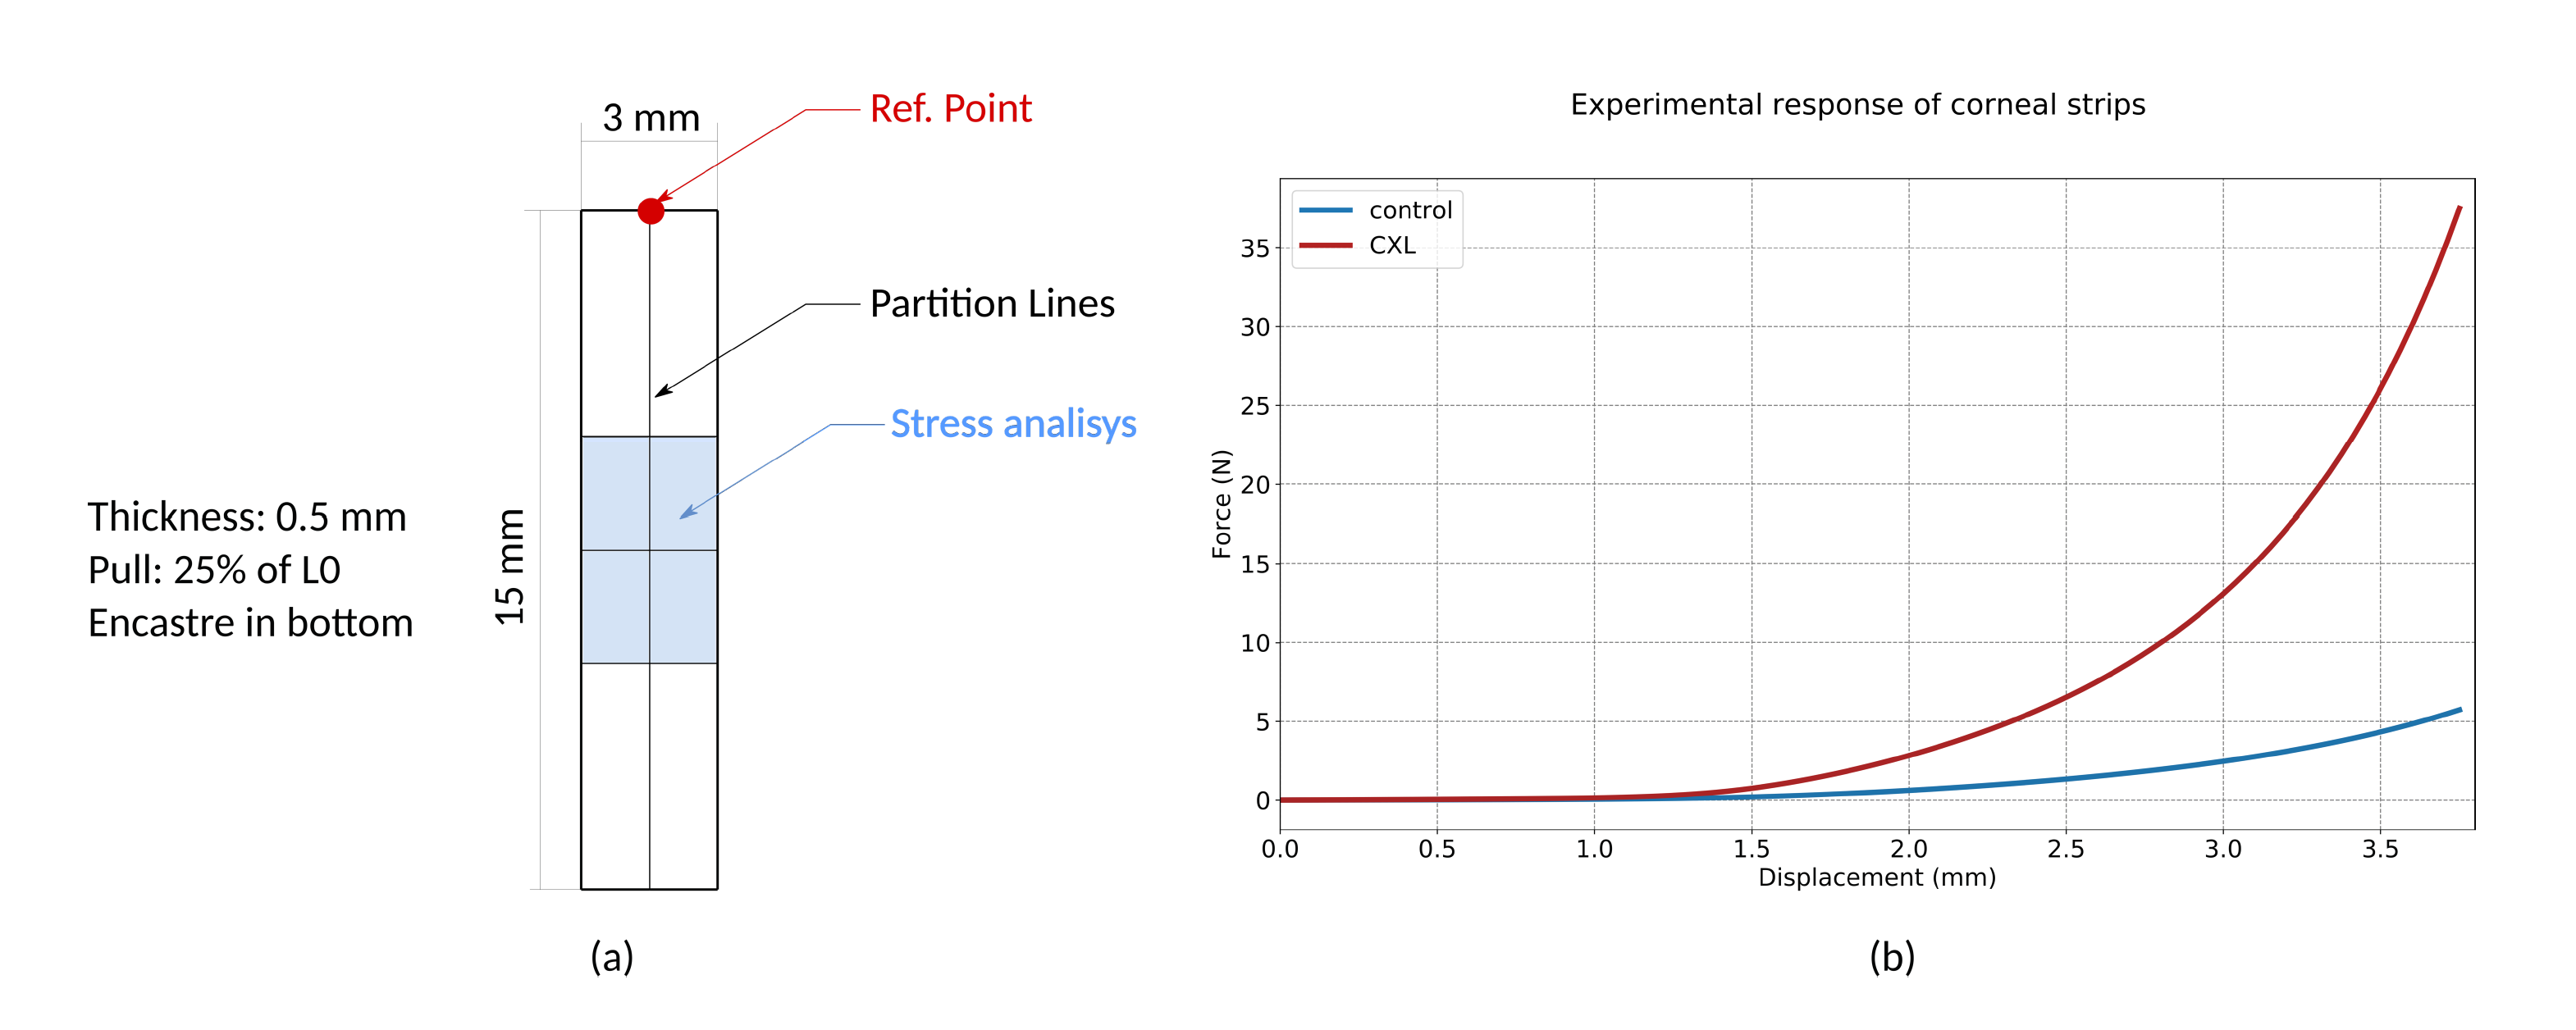
\includegraphics[width=0.9\linewidth]{pics/assignment_org}
   \caption{Shema of the sample in abaqus (a) and result of the experiment (b)}
    \label{fig:1}
  \end{figure}
  In Figure \ref{fig:1} in (b) we have two curves. One (control) shows the results form the experiment of a healthy person and the Other (clx) shows the result from a sample after chemical cross-linking (clx). The chemical cross-linking process should simulate the cornea of an elderly person. So with that data, we can model either a cornea of a healthy or an elderly person.
\newpage
\section{Methods}

\subsection{Sample and experimental data}
We created a model in Abaqus based on the requirements of the assignment as can be seen in Figure 1 in (a). We don't know the parameters of the sample jet. so we are estimating it and try if our sample is running. Therefore we used these parameters C10 = 5.5e-2, D = 1e-2, k1 = 65, k2 = 85, k = 0.2. Also, we rotate the sample as we want the force to be evenly distributed between the collagen strains. These strains are modeled within the formula. With the change of orientation in the \ang{30} direction the force are even on the strains.
\begin{figure}[!htb]
  \centering
  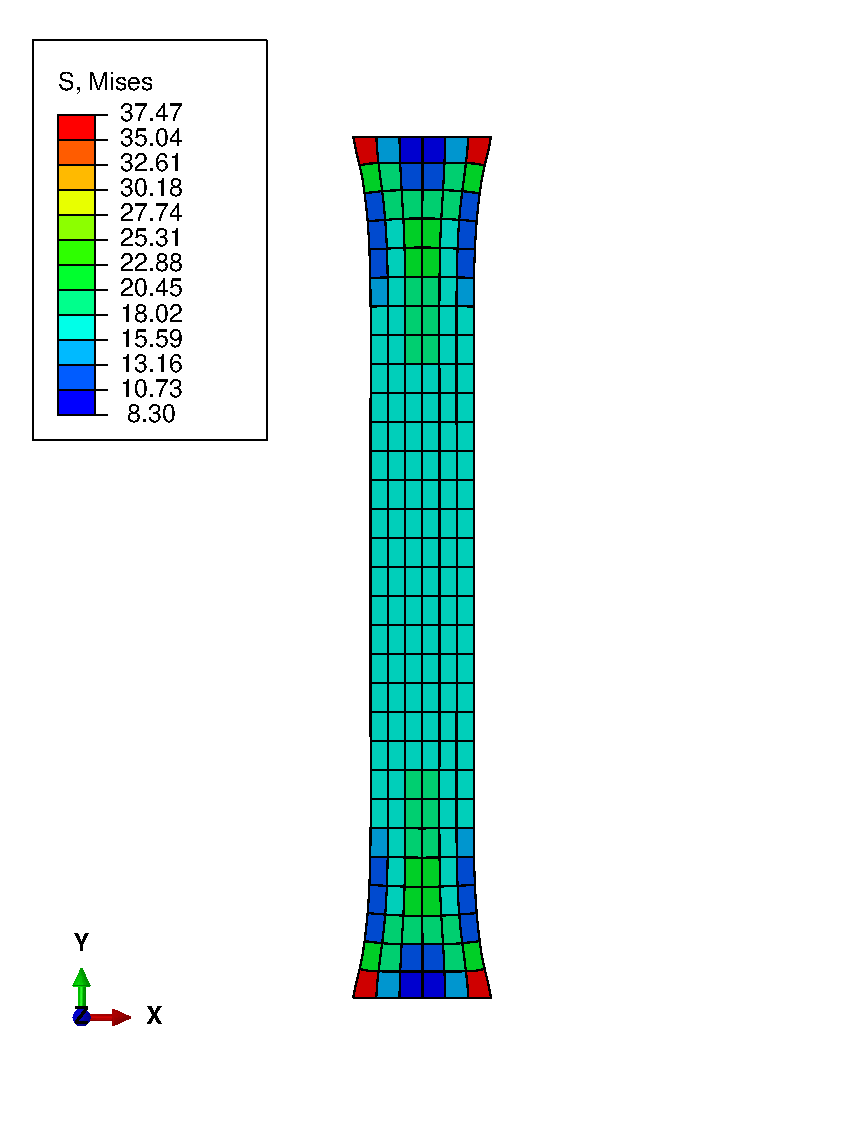
\includegraphics[width=0.5\linewidth]{pics/s_mises_45_bad}
 \caption{Stresses on the sample with not optimized parameters}
  \label{fig:2}
\end{figure}
Here with these parameters and the rotation, the even distribution is good across the sample. Later we will see the sample again with optimized parameters and what impact it has on the stresses of the model.
\pagebreak
\section{Results and Discussion}
\subsection{Optimization of the formula with $C_{10}$}
To determine the parameters of the formula to get an accurate representation of the real world sample an initial guess has to be made and then the result minimized to fit the control data from the experiment.
In this assignment, this is done via a python script. Abaqus can be run from the command line, with the reports and so on. So basically what is done is calling the job multiple times with different parameters for the material, the Holzapfel part. Giving a result with each run, the parameter can be changed to meet better the data from the experiment. Also, a cost function has to be implemented, as the minimizing function then tries to minimize the cost function.

In Figure \ref{fig:3} all optimizations are given. In this task, we especially try to optimize only the parameter $C_{10}$. Only from the specifics of this task, the result of optimizing the parameter $C_{10}$ cannot be good. The parameter $C_{10}$ displays only the neo hookien part of the stiffness matrix. In other ways, only the angle of the beginning of the slope can be changed with changing this parameter. $C_{10}$ only influences the beginning of the slope. So it is not a surprise that a bad optimized result is given.
\subsection{Optimization of the formula with $C_{10}, k_{1}, k_{2}$}
The parameters K1 and K2 give us better access to the specifics of the curve. As you can see in the result, the fit is very good for the control of the curve. What is done is actually not so difficult, only adding the 3 parameters to the cost function, using those as parameters are the only changes that have to be done to the python script.

The good fit with three parameters is excellent. it is now possible to have a very accurate sample in Abaqus for simulating different behaviors of the formula. The last output of the control values were C10: 0.031334, k1: 20.792526, k2: 64.772585. Actually, these results differ from our initial guess very much.

\begin{figure}[!htb]
  \centering
  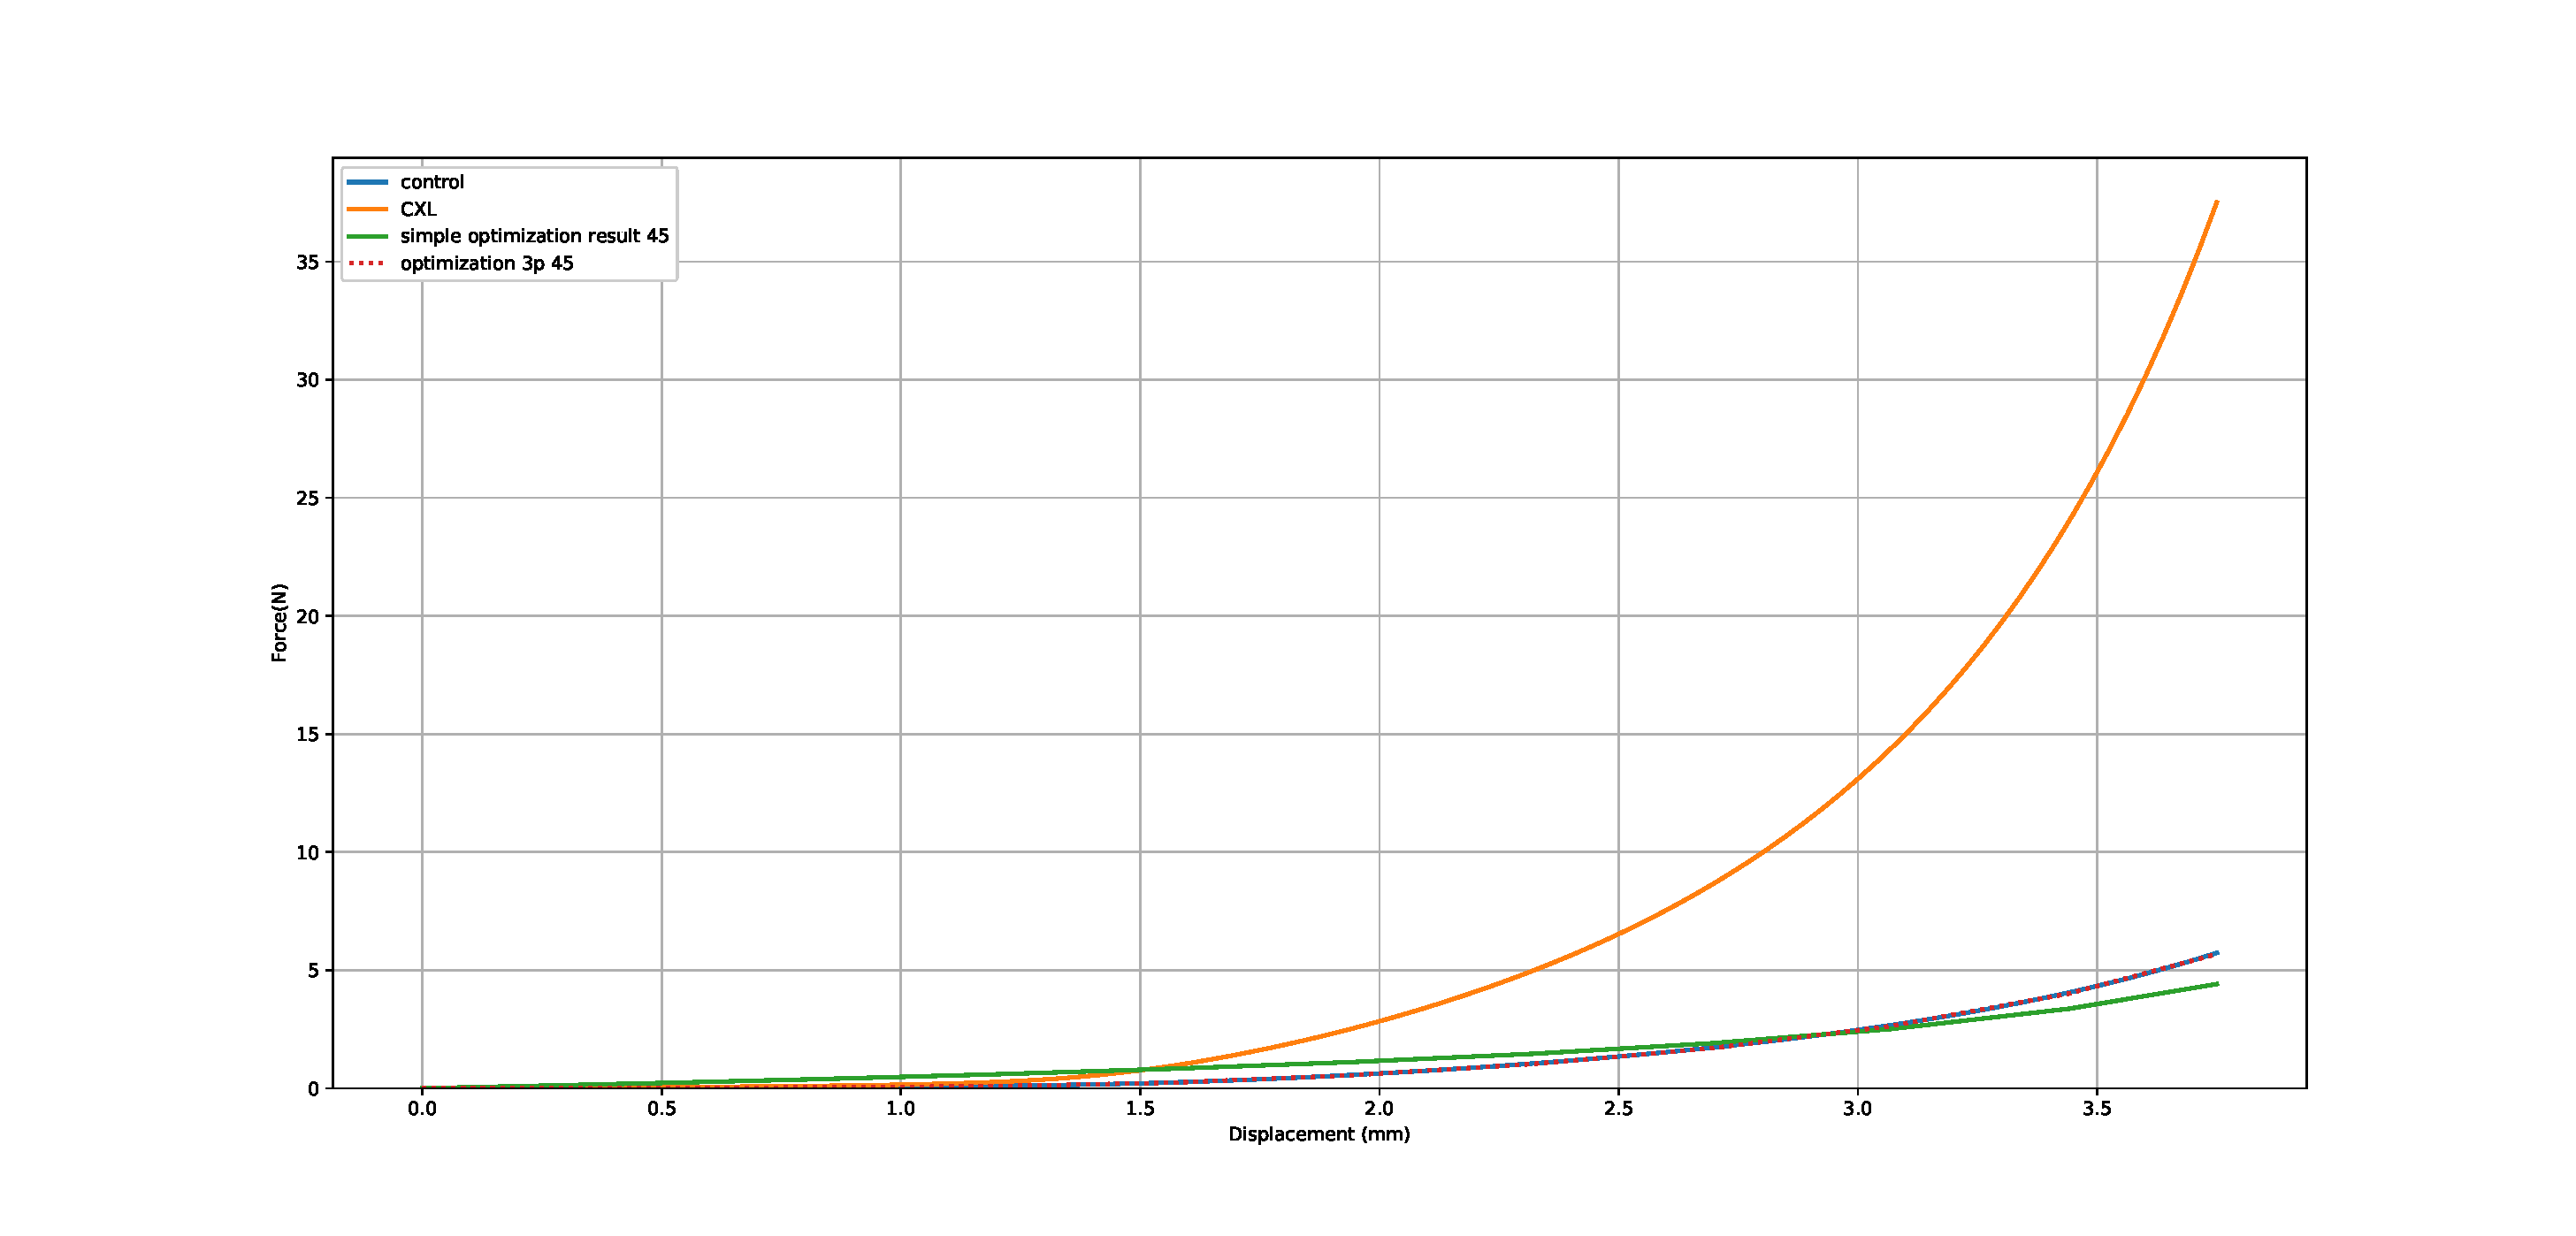
\includegraphics[width=0.8\linewidth]{pics/optimizations}
 \caption{Results of all optimizations}
  \label{fig:3}
\end{figure}
\pagebreak

\subsection{Stresses on sample with an angle of \ang{30} compared to \ang{45}}

\begin{figure}[!htb]
  \centering
  \begin{subfigure}{.5\textwidth}
    \centering
    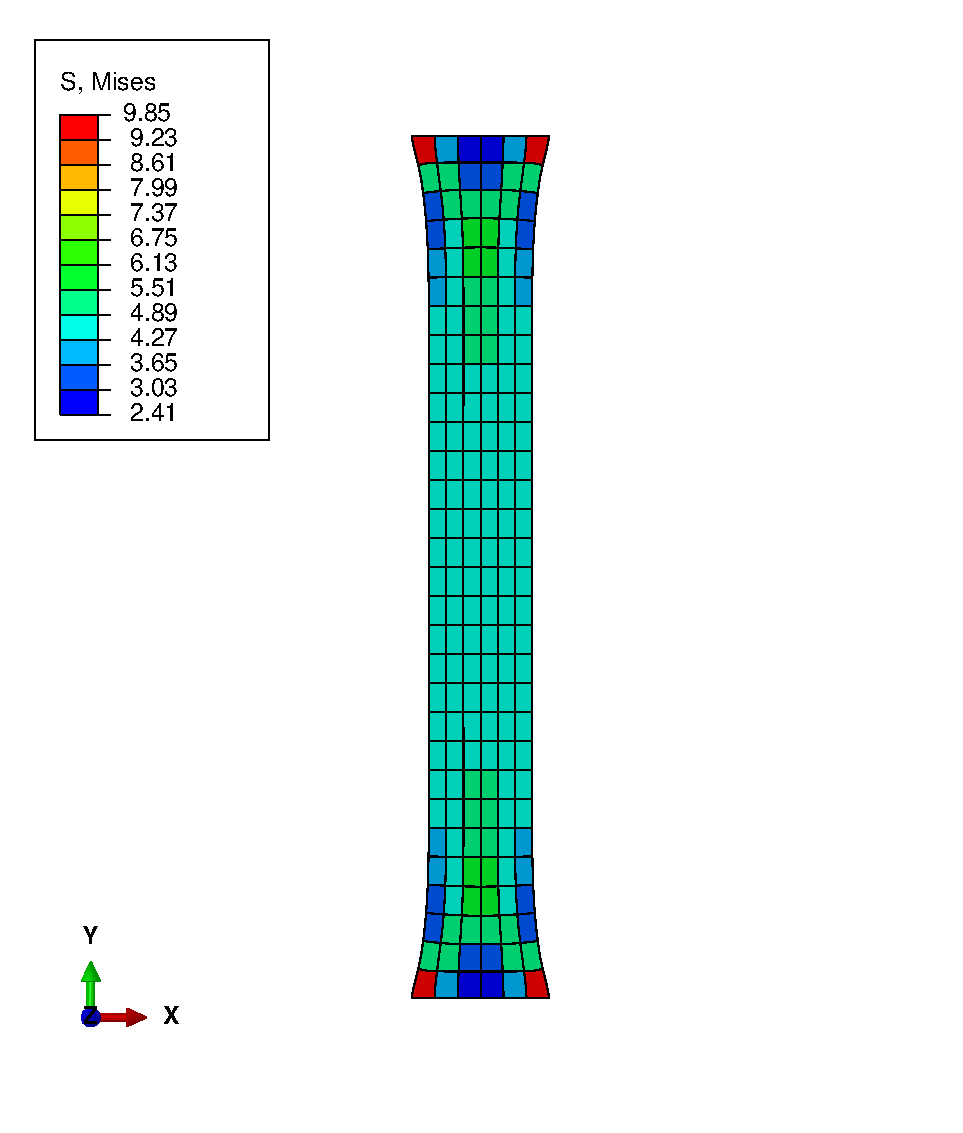
\includegraphics[width=0.95\linewidth]{pics/s_mises_45}
    \caption{Stresses with \ang{45}}
  \end{subfigure}%
  \begin{subfigure}{.5\textwidth}
    \centering
    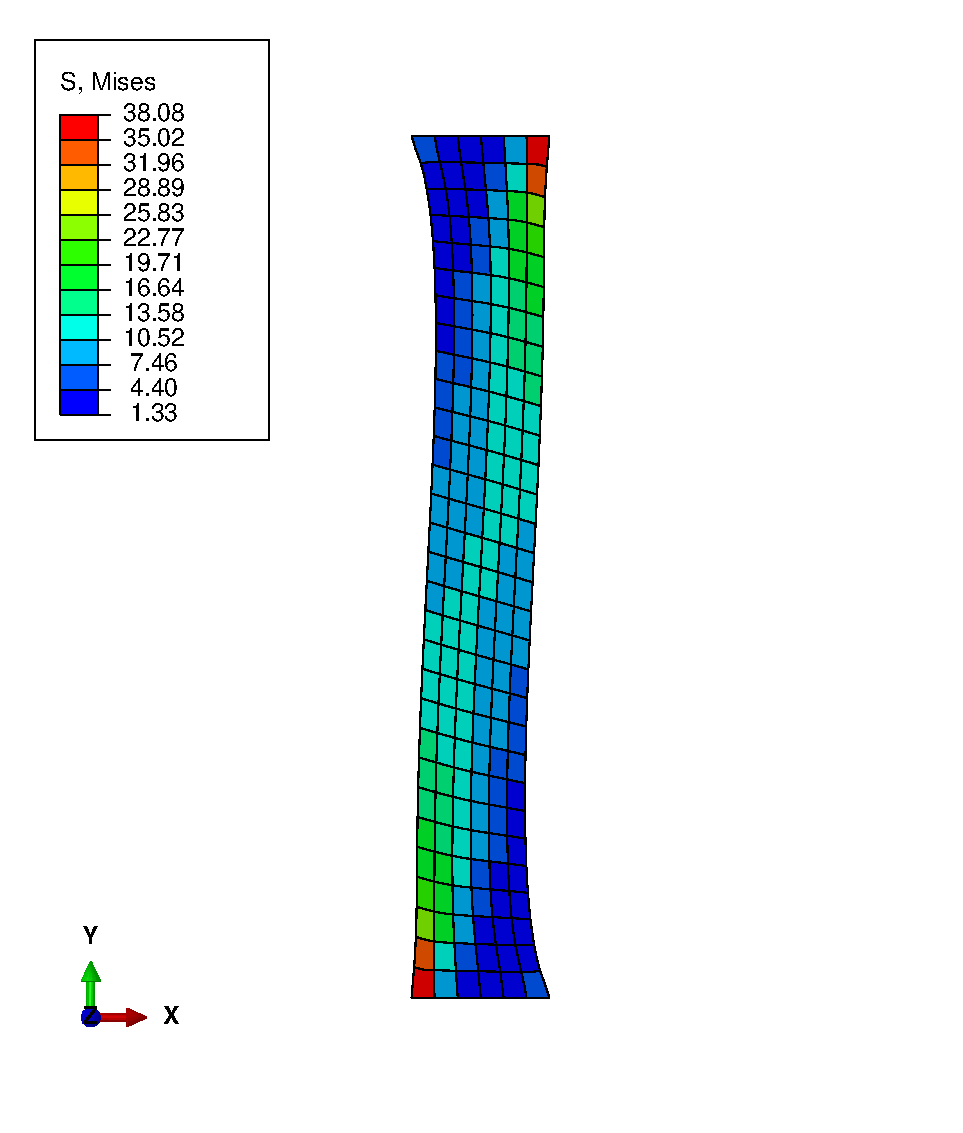
\includegraphics[width=0.95\linewidth]{pics/s_mises_30}
    \caption{Stresses with \ang{30}}
   \end{subfigure}
  \caption{Stresses on Sample}
  \label{fig:4}
\end{figure}
With the optimized values, a good estimate can be made. On the quarry plot, it looks quite similar, but the stresses on the simple are quite different compared to the real world. \ref{fig:2} shows high stresses and on the sample with the real values much lower stresses are seen.
We can now come to our actual experiment and for that, we change the rotation to \ang{30}. This is done by changing the datum on the sample by \ang{15}. The plot shows know that the stresses on the sample are not evenly distributed as seen before in the \ang{45} sample. The \ang{45} sample shows very well how the stresses are evenly over the sample because the forces on the collagen fibers are almost equally as we pull in this direction. The \ang{30} sample shows that these forces are more distributed on the side of the fibers closer to the original \ang{45} direction. Even the direction of the fibers are not aligned accordingly, a twist of forces is visible on the \ang{30} sample.
\pagebreak
\begin{figure}[!htb]
  \centering
  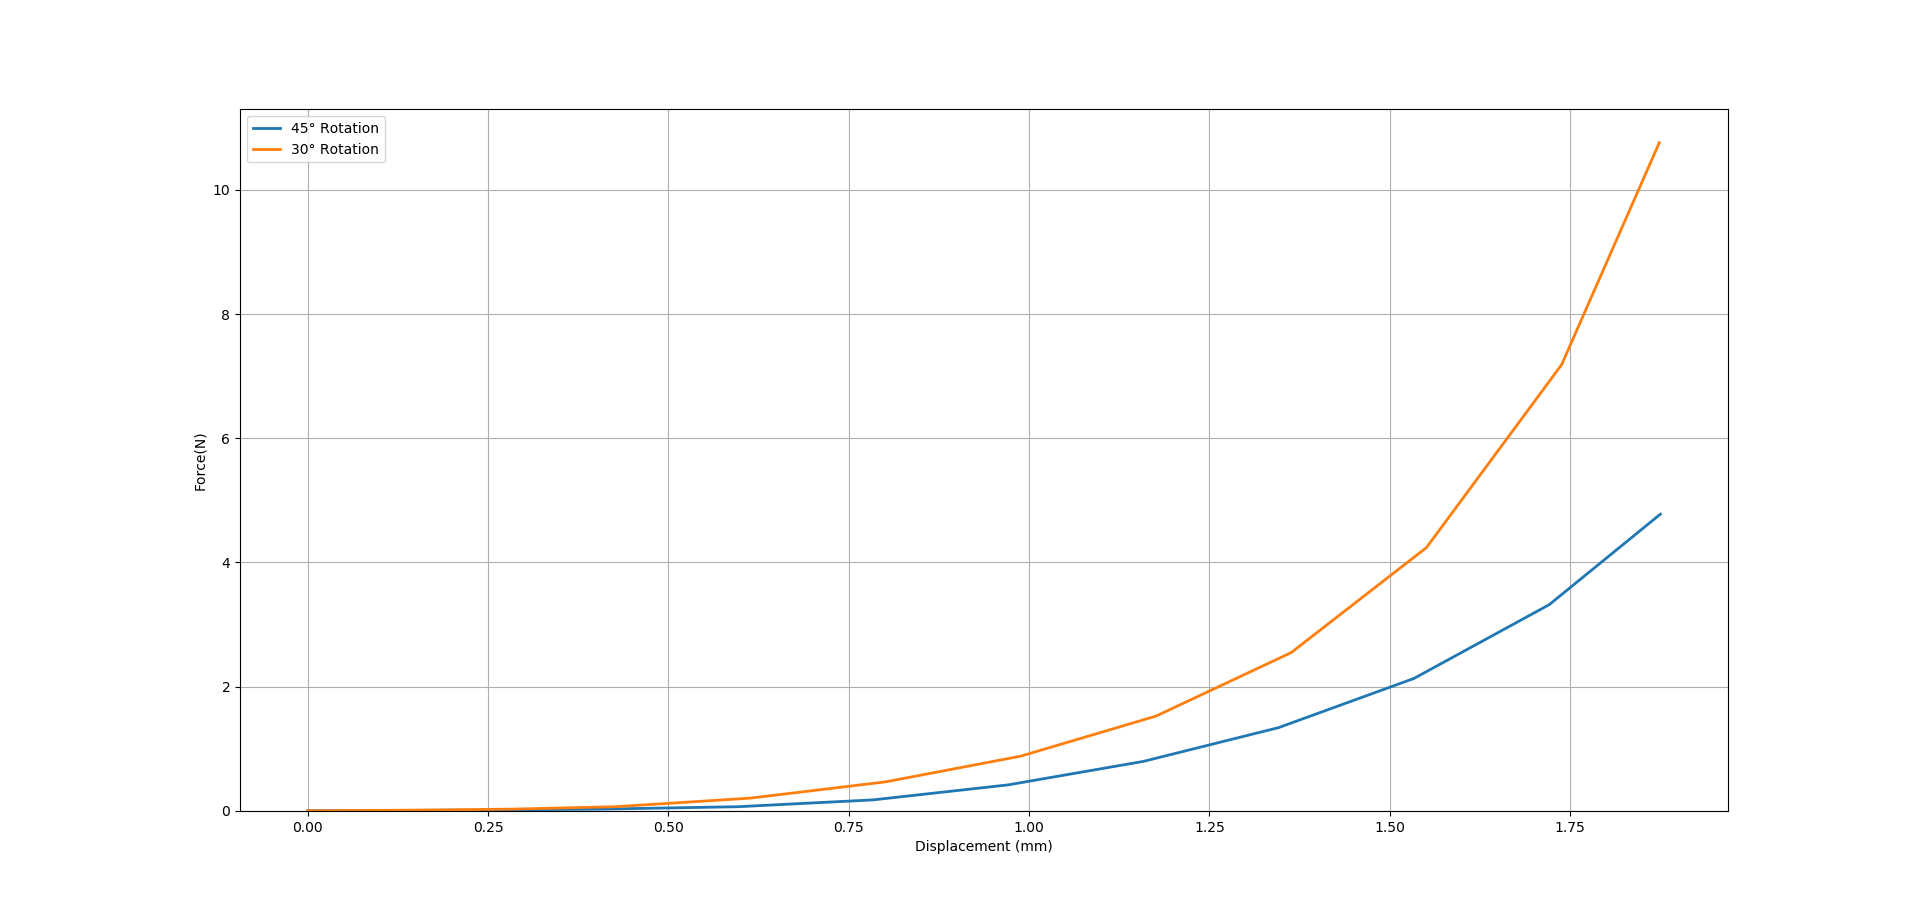
\includegraphics[width=1.0\linewidth]{pics/rotations}
 \caption{Stresses on central point of sample compared}
  \label{fig:5}
\end{figure}
Plotting the stresses on the central point of the shape gives us a comparison of how the forces are applied to the sample. It is interesting that for the \ang{30} sample more force has to be given to the entity to reach the same displacement as with the \ang{45} sample. The reason why the \ang{30} uses more energy is that the fibers first have to change into the direction of force where it is pulled from. This is not required for the fibers aligned in the \ang{45} direction. In short, aligned with the direction of the force uses energy.

\section{Conclusion}
This assignment was very interdisciplinary in the way of working with. So many skills are necessary, not only understanding a cost function, also knowledge is required for understanding the minimization algorithm. Not it is only the programmatical part also knowledge in forces, hyperelasticity and the behavior of it is required. Using that knowledge to feed the Holzapfel formula is a large amount of work. The actual analyses are not even made. What the goal of this assignment was is the way of how we get from the real world to our numerical model in Abaqus. However, working with this assignment was very intense and used a lot of time, and was very interesting. The time spent with this assignment was actually funny because you only see a result in every step one has made.

\begin{thebibliography}{9}
  \bibitem{Holzapfel-Gasser-Ogden} 
  https://www.sharcnet.ca/Software/Abaqus610/Documentation/docs/v6.10/books/stm/default.htm?startat=ch04s06ath125.html\#stm-mat-anisohyperelastic-holzapfel
\end{thebibliography}


\end{document}